
\documentclass[12pt]{article}

\usepackage{amsmath}
\allowdisplaybreaks
\usepackage{amsthm}
\usepackage{amssymb}
\usepackage[colorlinks=true]{hyperref}
\usepackage{tikz}
\usepackage{natbib}
\usepackage[margin=2cm]{geometry}

\usetikzlibrary{bayesnet}

\newtheorem{lemma}{Lemma}
\newtheorem{theorem}{Theorem}

\title{Derivation of the Kalman filter equations}
\author{Joaquín Rapela}

\begin{document}

\maketitle

\begin{theorem}
	\label{thm:kalmanFilterEqs}

    Given the linear dynamical systems model

    \begin{alignat*}{2}
        \mathbf{x}_{t+1}&=A_t\mathbf{x}_t+\mathbf{w}_t&\quad&\text{with }\mathbf{w}_t\sim N(0,Q_t)\\
        \mathbf{y}_t&=B_t\mathbf{x}_t+\mathbf{v}_t&&\text{with }\mathbf{v}_t\sim N(0,R_t)\\
        \mathbf{x}_0&\sim N(\mathbf{m}_0,V_0)&&
    \end{alignat*}

    \noindent (represented in Fig.~\ref{fig:ldsModel}), then the predictive
    distribution, $p(\mathbf{x}_t|\mathbf{y}_1,\ldots,\mathbf{y}_{t-1})$, and
    the filtering distribution,
    $p(\mathbf{x}_t|\mathbf{y}_1,\ldots,\mathbf{y}_t)$, are

    \begin{align*}
        p(\mathbf{x}_t|\mathbf{y}_1,\ldots,\mathbf{y}_{t-1})&=N(\mathbf{x}_t|\mathbf{x}_{t|t-1},P_{t|t-1})\\
        p(\mathbf{x}_t|\mathbf{y}_1,\ldots,\mathbf{y}_t)&=N(\mathbf{x}_t|\mathbf{x}_{t|t},P_{t|t})
    \end{align*}

    \noindent with

    \begin{align}
        \mathbf{x}_{t|t-1}&=A_{t-1}\mathbf{x}_{t-1|t-1}\label{eq:xtGtm1}\\
        P_{t|t-1}&=A_{t-1}P_{t-1|t-1}A_{t-1}^\intercal+Q_{t-1}\label{eq:PtGtm1}\\
        \hat{\mathbf{y}}_{t|t-1}&\triangleq E\{\mathbf{y}_t|\mathbf{y}_1,\ldots,\mathbf{y}_{t-1}\}=B_t\mathbf{x}_{t|t-1}\label{eq:ytGtm1}\\
        \mathbf{z}_t&\triangleq\mathbf{y}_t-\hat{\mathbf{y}}_{t|t-1}\nonumber\\
        S_t&\triangleq \text{Cov}\{\mathbf{z}_t|\mathbf{y}_1,\ldots,\mathbf{y}_{t-1}\}=B_tP_{t|t-1}B_t^\intercal+R_t\label{eq:St}\\
        \mathbf{x}_{t|t}&=\mathbf{x}_{t|t-1}+K_t\mathbf{z}_t\label{eq:xtGt}\\
        \mathbf{P}_{t|t}&=(I-K_tB_t)P_{t|t-1}\label{eq:PtGt}\\
        \mathbf{K}_t&=P_{t|t-1}B_t^\intercal S_t^{-1}\label{eq:Kt}\\
        \mathbf{x}_{0|0}&=\mathbf{m}_0\label{eq:x0G0}\\
        P_{0|0}&=V_0\label{eq:P0G0}
    \end{align}
\end{theorem}

The following proof adds a few details to that given in Section 4.3.1 of
\citet{durbinAndKoopman12}.

\begin{proof}
    Call $Y_t=\{\mathbf{y}_1,\ldots,\mathbf{y}_t\}$, then

    \begin{align}
        \mathbf{x}_{t|t-1}&=E\{\mathbf{x}_t|Y_{t-1}\}=E\{A_{t-1}\mathbf{x}_{t-1}+\mathbf{w}_{t-1}|Y_{t-1}\}\nonumber\\
                          &=A_{t-1}E\{\mathbf{x}_{t-1}|Y_{t-1}\}+E\{\mathbf{w}_{t-1}|Y_{t-1}\}\nonumber\\
                          &=A_{t-1}\mathbf{x}_{t-1|t-1}+E\{\mathbf{w}_{t-1}\}=A_{t-1}\mathbf{x}_{t-1|t-1}\label{eq:p1n1}
    \end{align}
	This proves Eq.~\ref{eq:xtGtm1}.

    \begin{align}
        \mathbf{P}_{t|t-1}&=\text{Cov}\{\mathbf{x}_t|Y_{t-1}\}=E\{(\mathbf{x}_t-\mathbf{x}_{t|t-1})(\mathbf{x}_t-\mathbf{x}_{t|t-1})^\intercal|Y_{t-1}\}\nonumber\\
                          &=E\{\left(A_{t-1}\mathbf{x}_{t-1}+w_{t-1}-A_{t-1}\mathbf{x}_{t-1|t-1}\right)\left(A_{t-1}\mathbf{x}_{t-1}+w_{t-1}-A_{t-1}\mathbf{x}_{t-1|t-1}\right)^\intercal|Y_{t-1}\}\nonumber\\
                          &=E\{\left(A_{t-1}(\mathbf{x}_{t-1}-\mathbf{x}_{t-1|t-1})+w_{t-1}\right)\left(A_{t-1}(\mathbf{x}_{t-1}-\mathbf{x}_{t-1|t-1})+w_{t-1}\right)^\intercal|Y_{t-1}\}\nonumber\\
                          &=A_{t-1}E\{(\mathbf{x}_{t-1}-\mathbf{x}_{t-1|t-1})(\mathbf{x}_{t-1}-\mathbf{x}_{t-1|t-1})^\intercal|Y_{t-1}\}A_{t-1}^\intercal+\nonumber\\
                          &\qquad E\{w_{t-1}(\mathbf{x}_{t-1}-\mathbf{x}_{t-1|t-1})^\intercal|Y_{t-1}\}A_{t-1}^\intercal+\nonumber\\
                          &\qquad A_{t-1}E\{(\mathbf{x}_{t-1}-\mathbf{x}_{t-1|t-1})w_{t-1}^\intercal|Y_{t-1}\}+\nonumber\\
                          &\qquad E\{w_{t-1}w_{t-1}^\intercal|Y_{t-1}\}\nonumber\\
                          &=A_{t-1}E\{(\mathbf{x}_{t-1}-\mathbf{x}_{t-1|t-1})(\mathbf{x}_{t-1}-\mathbf{x}_{t-1|t-1})^\intercal|Y_{t-1}\}A_{t-1}^\intercal+\nonumber\\
                          &\qquad E\{w_{t-1}|Y_{t-1}\}E\{(\mathbf{x}_{t-1}-\mathbf{x}_{t-1|t-1})^\intercal|Y_{t-1}\}A_{t-1}^\intercal+\nonumber\\
                          &\qquad A_{t-1}E\{(\mathbf{x}_{t-1}-\mathbf{x}_{t-1|t-1})|Y_{t-1}\}E\{w_{t-1}^\intercal|Y_{t-1}\}+\nonumber\\
                          &\qquad E\{w_{t-1}w_{t-1}^\intercal\}\label{eq:p1n2}\\
                          &=A_{t-1}P_{t-1|t-1}A_{t-1}^\intercal+Q_{t-1}\label{eq:p1n3}
    \end{align}
	This proves Eq.~\ref{eq:PtGtm1}.

    \begin{align}
        \hat{\mathbf{y}}_{t|t-1}&=E\{\mathbf{y}_t|Y_{t-1}\}=E\{B_t\mathbf{x}_t+\mathbf{v}_t|Y_{t-1}\}=B_tE\{\mathbf{x}_t|Y_{t-1}\}+E\{\mathbf{v}_t|Y_{t-1}\}\nonumber\\
                                &=B_t\mathbf{x}_{t|t-1}+E\{\mathbf{v}_t\}=B_t\mathbf{x}_{t|t-1}\nonumber
    \end{align}
	This proves Eq.~\ref{eq:ytGtm1}.

    Because

    \begin{align}
        \mathbf{z}_t&=\mathbf{y}_t-\hat{\mathbf{y}}_{t|t-1}=B_t\mathbf{x}_t+\mathbf{v}_t-B_t\mathbf{x}_{t|t-1}=B_t(\mathbf{x}_t-\mathbf{x}_{t|t-1})+\mathbf{v}_t\label{eq:ztProof}
    \end{align}

    \noindent $Y_{t-1}$ and $\mathbf{z}_t$ are fixed if and only if $Y_t$ is
    fixed\footnote{If we now $Y_{t-1}$ and $\mathbf{z}_t$, then we know
    $\hat{\mathbf{y}}_{t|t-1}$ and $\mathbf{z}_t$, then (by the first equality
    in Eq.~\ref{eq:ztProof}) we know $\mathbf{y}_t$, thus we know $Y_t$. Also, if we
    know $Y_t$, we know $\hat{\mathbf{y}}_{t|t-1}$ and $\mathbf{y}_t$ and (by
    the first equality in Eq.~\ref{eq:ztProof}) we know $\mathbf{z}_t$.}. Then

    \begin{align}
        \mathbf{x}_{t|t}&=E\{\mathbf{x}_t|Y_t\}=E\{\mathbf{x}_t|Y_{t-1},\mathbf{z}_t\}\nonumber\\
                        &=E\{\mathbf{x}_t|Y_{t-1}\}+\text{Cov}\left(\mathbf{x}_t,\mathbf{z}_t|Y_{t-1}\right)\text{Cov}\left(\mathbf{z}_t|Y_{t-1}\right)^{-1}\mathbf{z}_t\label{eq:xtGtTmp}\\
        \text{Cov}\left(\mathbf{x}_t,\mathbf{z}_t|Y_{t-1}\right)&=\text{Cov}\left(\mathbf{x}_t,B_t(\mathbf{x}_t-\mathbf{x}_{t|t-1})+\mathbf{v}_t|Y_{t-1}\right)\nonumber\\
                                                                &=E\{(\mathbf{x}_t-\mathbf{x}_{t|t-1})(B_t(\mathbf{x}_t-\mathbf{x}_{t|t-1})+\mathbf{v}_t)^\intercal|Y_{t-1}\}\nonumber\\
                                                                &=E\{(\mathbf{x}_t-\mathbf{x}_{t|t-1})(\mathbf{x}_t-\mathbf{x}_{t|t-1})^\intercal|Y_{t-1}\}B_t^\intercal\nonumber\\
                                                                &\qquad +E\{(\mathbf{x}_t-\mathbf{x}_{t|t-1})\mathbf{v}_t^\intercal|Y_{t-1}\}\nonumber\\
                                                                &=P_{t|t-1}B_t^\intercal\label{eq:covXZ}\\
        S_t=\text{Cov}\left(\mathbf{z}_t|Y_{t-1}\right)&=E\{\mathbf{z}_t\mathbf{z}_t^\intercal|Y_{t-1}\}\nonumber\\
                                                       &=E\{\left(B_t(\mathbf{x}_t-\mathbf{x}_{t|t-1})+\mathbf{v}_t\right)\left(B_t(\mathbf{x}_t-\mathbf{x}_{t|t-1})+\mathbf{v}_t\right)^\intercal|Y_{t-1}\}\nonumber\\
                                                       &=B_tE\{\left(\mathbf{x}_t-\mathbf{x}_{t|t-1}\right)\left(\mathbf{x}_t-\mathbf{x}_{t|t-1}\right)^\intercal|Y_{t-1}\}B_t^\intercal\nonumber\\
                                                       &\qquad +E\{\mathbf{v}_t\mathbf{v_t}^\intercal|Y_{t-1}\}\nonumber\\
                                                       &=B_tP_{t|t-1}B_t^\intercal+R_t\label{eq:covZ}
    \end{align}
	This proves Eq.~\ref{eq:St}.

    Combining Eqs.~\ref{eq:xtGtTmp}, \ref{eq:covXZ} and~\ref{eq:covZ} we obtain

    \begin{align}
        \mathbf{x}_{t|t}&=\mathbf{x}_{t|t-1}+P_{t|t-1}B_t^\intercal
        S_t^{-1}\mathbf{z}_t\nonumber\\
                        &=\mathbf{x}_{t|t-1}+K_t\mathbf{z}_t\quad\text{with } K_t=P_{t|t-1}B_t^\intercal S_t^{-1}\nonumber\\
        P_{t|t}&=\text{Cov}(\mathbf{x}_t|Y_t)=\text{Cov}(\mathbf{x}_t|Y_{t-1},\mathbf{z}_t)=P_{t|t-1}-P_{t|t-1}B_t^\intercal S_t^{-1}B_tP_{t|t-1}\nonumber\\
               &=\left(I-P_{t|t-1}B_t^\intercal S_t^{-1}B_t\right)P_{t|t-1}=\left(I-K_tB_t\right)P_{t|t-1}\label{eq:PtGtProof}
    \end{align}
	This proves Eqs.~\ref{eq:xtGt}, \ref{eq:PtGt} and~\ref{eq:Kt}.

	Using Eqs.~\ref{eq:x0G0} and~\ref{eq:P0G0} in Eqs.~\ref{eq:xtGtm1} and~\ref{eq:PtGtm1} we obtain

    \begin{align*}
        \mathbf{x}_{1|0}&=A_0\mathbf{x}_{0|0}=A_0\mathbf{m}_0\\
        \mathbf{P}_{1|0}&=A_0P_{0|0}A_0^\intercal+Q_0=A_0V_0A_0^\intercal+Q_0
    \end{align*}

	If Eqs.~\ref{eq:x0G0} and~\ref{eq:P0G0} are correct, then the density of $\mathbf{x}_1$ should be $p(\mathbf{x}_1)=\mathcal{N}(\mathbf{x}_1|\mathbf{x}_{1|0},P_{1|0})$. We now calculate this density using the linear dynamical system model in Theorem~\ref{thm:kalmanFilterEqs}.

    \begin{align}
		p(\mathbf{x}_1)&=\int p(\mathbf{x}_1,\mathbf{x}_0)d\mathbf{x}_0=\int p(\mathbf{x}_1|\mathbf{x}_0)p(\mathbf{x}_0)d\mathbf{x}_0=\int\mathcal{N}(\mathbf{x}_1|A_0\mathbf{x}_0,Q_0)\mathcal{N}(\mathbf{x}_0|\mathbf{m}_0,V_0)d\mathbf{x}_0\nonumber\\
		               &=\mathcal{N}(\mathbf{x}_1|A_0\mathbf{m}_0,A_0V_0A_0^\intercal+Q_0)=\mathcal{N}(\mathbf{x}_1|\mathbf{x}_{1|0},\mathbf{P}_{1|0})\label{eq:px1}
    \end{align}
	This proves Eqs.~\ref{eq:x0G0} and~\ref{eq:P0G0}.

\end{proof}

Notes:
\begin{enumerate}
    \item the first equality in Eq.~\ref{eq:p1n1} holds because
        $\mathbf{w}_{t-1}$ is independent of $Y_{t-1}$.
    \item the second and third terms in Eq.~\ref{eq:p1n2} hold because
        $w_{t-1}$ is independent of $x_{t-1}$ given $Y_{t-1}$.
    \item Eq.~\ref{eq:p1n3} holds because
        $E\{\mathbf{x}_{t-1}-\mathbf{x}_{t-1|t-1}|Y_{t-1}\}=0$.
    \item the last equality in Eq.~\ref{eq:xtGtTmp} follows from Eq.~\ref{eq:conditionalMean} in
        Lemma~\ref{lemma:conditionalGaussians}
    \item the last equality in Eq.~\ref{eq:covXZ} holds because $\mathbf{x}_t$
        in independent (and therefore uncorrelated) of $\mathbf{v}_t$.
    \item the second equality of Eq.~\ref{eq:covZ} uses Eq.~\ref{eq:ztProof}.
    \item the third equality of Eq.~\ref{eq:covZ} holds because $\mathbf{x}_t$
        is independent of $\mathbf{v}_t$ given $Y_{t-1}$.
    \item the last equality of Eq.~\ref{eq:covZ} holds because $\mathbf{v}_t$
        is independent of $Y_{t-1}$.
	\item in the third equality of Eq.~\ref{eq:PtGtProof} we used Eq.~\ref{eq:conditionalCov} in Lemma~\ref{lemma:conditionalGaussians}
	with $\mathbf{x}=\mathbf{x}_t|Y_{t-1}$ and $\mathbf{y}=\mathbf{z}_t|Y_{t-1}$ giving

		\begin{align*}
			\Sigma_{x|y}&=\Sigma_{\mathbf{x}_t|\mathbf{z}_t,Y_{t-1}}=\Sigma_{\mathbf{x}_t|Y_t}=P_{t|t}\\
			\Sigma_{xx}&=\Sigma_{\mathbf{x}_t|Y_{t-1}}=P_{t|t-1}\\
			\Sigma_{xy}&=\Sigma_{\mathbf{x}_t\mathbf{z}_t|Y_{t-1}}=\text{Cov}(\mathbf{x}_t,\mathbf{z}_t|Y_{t-1})=P_{t|t-1}B_t^\intercal\\
			\Sigma_{yy}&=\Sigma_{\mathbf{z}_t\mathbf{z}_t|Y_{t-1}}=\text{Cov}(\mathbf{z}_t|Y_{t-1})=S_t\\
                        &\text{thus}\\
            P_{t|t}&=P_{t|t-1}-P_{t|t-1}B_t^\intercal S_t^{-1}B_tP_{t|t-1}
		\end{align*}
	\item in the fourth equality of Eq.~\ref{eq:px1} we used Lemma~\ref{lemma:linearModelGaussianLatents}.

\end{enumerate}

\begin{figure}
    \centering
    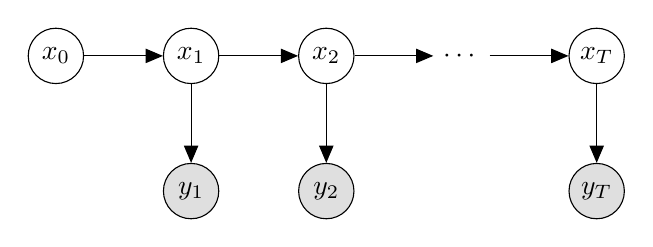
\begin{tikzpicture}[node distance=2.5cm and 1.8cm]

  % Nodes for hidden states
  \node[latent]              (x0) {$x_0$};
  \node[latent, right=of x0] (x1) {$x_1$};
  \node[latent, right=of x1] (x2) {$x_2$};
  \node[latent, right=of x2, draw=none] (xD) {$\cdots$};
  \node[latent, right=of xD] (xT) {$x_T$};

  % Nodes for observations
  \node[obs, below=of x1] (y1) {$y_1$};
  \node[obs, below=of x2] (y2) {$y_2$};
  \node[obs, below=of xT] (yT) {$y_T$};

  % Edges between hidden states
  \edge {x0} {x1};
  \edge {x1} {x2};
  \edge {x2} {xD};
  \edge {xD} {xT};

  % Emission edges
  \edge {x1} {y1};
  \edge {x2} {y2};
  \edge {xT} {yT};

\end{tikzpicture}

    \caption{Graphical models for our linear dynamical system in
    Theorem~\ref{thm:kalmanFilterEqs}.}
    \label{fig:ldsModel}
\end{figure}

\documentclass[12pt]{article}

\usepackage{amsmath}
\usepackage{theorem}

\newtheorem{theorem}{Theorem}

\title{Conditional distribution for jointly normal Gaussian random variables}
\author{Joaquín Rapela}

\begin{document}

\maketitle

\begin{theorem}

    Let $\mathbf{x}$ and $\mathbf{y}$ be jointly normally-distributed random
    vectors with

    \begin{align*}
        E\left\{\left(\begin{array}{c}
                          \mathbf{x}\\
                          \mathbf{y}
                      \end{array}\right)\right\}&=\left(\begin{array}{c}
                                                           \boldsymbol{\mu}_x\\
                                                           \boldsymbol{\mu}_y
                                                       \end{array}\right)\\
        \text{Cov}\left\{\left(\begin{array}{c}
                                   \mathbf{x}\\
                                   \mathbf{y}
                               \end{array}\right)\right\}&=\left(\begin{array}{cc}
                                                                     \Sigma_{xx} & \Sigma_{xy} \\
                                                                     \Sigma_{yx} & \Sigma_{yy} \\
                                                                  \end{array}\right)
    \end{align*}

    \noindent where $\Sigma_{yy}$ is assumed to be non-singular.
    %
    Then the conditional distribution of $\mathbf{x}$ given $\mathbf{y}$ is
    normal with mean vector

    \begin{align*}
        \text{E}\{\mathbf{x}|\mathbf{y}\}=\boldsymbol{\mu}_x+\Sigma_{xy}\Sigma_{yy}^{-1}(\mathbf{y}-\boldsymbol{\mu}_y)
    \end{align*}

    \noindent and covariance matrix

    \begin{align*}
        \text{Cov}\{\mathbf{x}|\mathbf{y}\}=\Sigma_{xx}-\Sigma_{xy}\Sigma_{yy}^{-1}\Sigma_{yx}
    \end{align*}
\end{theorem}

\end{document}


\bibliographystyle{apalike}
\bibliography{linearDynamicalSystems}

\end{document}
